\section{Risposta in frequenza}
Usando in circuito in figura (\ref{f:setup}) si è misurata la tensione $V_{out}$ al variare della frequenza del generatore d'onda, utilizzando per entrambe le misure l'oscilloscopio. La tensione in ingresso (picco-picco) è stata mantenuta sempre a \SI{0.79(2)}{\V}
Si sono effettuati tre fit per ottenere i valori delle frequenze di taglio che risultano essere:\\
$f_{inf}= \SI{60.4(9) }{\Hz} $\\
$f_{sup}= \SI{93(2) }{\kHz} $\\
Tali valori sono stati individuati dalle intersezioni delle due rette oblique con quella orizzontale direttamente dal grafico in figura(\ref{f:guadagno_freq}).

\begin{figure}[h]
	\centering
	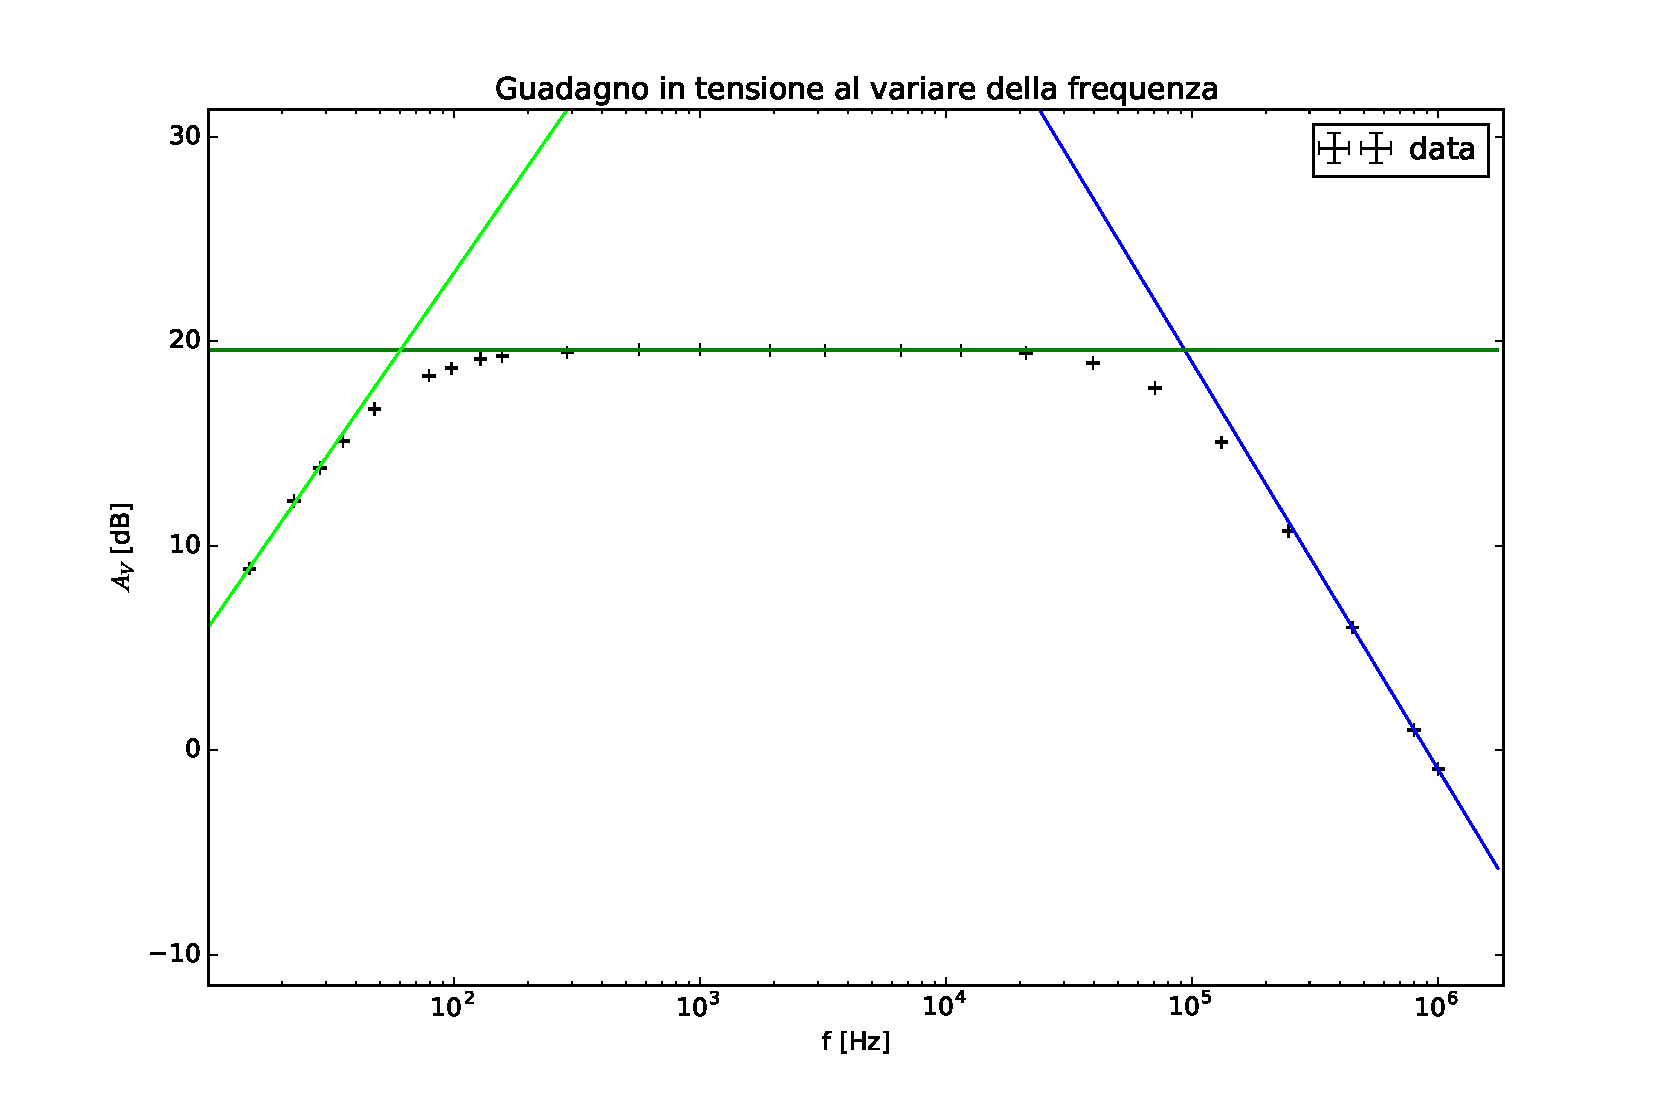
\includegraphics[scale=0.6]{guadagno_freq.pdf}
	\caption{Guadagno in tensione del circuito al variare della frequenza del segnale $V_{in}$}
	\label{f:guadagno_freq}
\end{figure}

Il fit della zona centrale del grafico (\ref{f:guadagno_freq}) è stato eseguito con una funzione costante $A_V =b$ ed inoltre si è limitato il set di dati usato per tale fit alla regione con $ \SI{500}{\Hz} \leq f \leq \SI{11}{\kHz}$. Si è ottenuto:\\
$b= \SI{19.57 \pm 0.02}{\dB}$ \\
$\chi^2= 1.32$ ($4$ DoF, $p_{\chi^2>1.32} = 0.85)$\\
I fit delle rette oblique sono stati eseguiti in entrambi i casi con una funzione del tipo$A_V = a\log_{10} f/_{\si{\Hz}} +b$. Per la retta di sinistra sono stati considerati nel fit solo i primi tre punti, in quanto ancora così si può notare come il fit lineare non sia una buona approssimazione, segno dell'essere troppo vicini alla frequenza di taglio. I valori ottenuti dal fit sono :\\
$a= \SI{17.3(2)}{\dB\per\deca} $ \\
$b=-11.3 \pm 0.3 dB $ \\
$\chi^2= 14.9$ ($1$ DoF, $p_{\chi^2>14.9} = 0.0001)$\\
Per la retta di destra si sono considerati i valori di $f> \SI{350}{\kHz}$ e si è ottenuto :\\
$a= \SI{-19.9(2)}{\dB\per\deca} $ \\
$b= 118 \pm 1 dB $ \\
$\chi^2= 1.2$ ($1$ DoF, $p_{\chi^2>1.2} = 0.27)$\\

La frequenza di taglio inferiore si pensa sia riconducibile alla frequenza di taglio del filtro tra $C_{in}$ e il parallelo $R_{parallelo }= R_1 \paral R_2 $, infatti si ha $f_{inf,att}= \frac{1}{2 \pi R_{parallelo}C_{in}}= \SI{45.2 \pm 1.8}{\Hz}$. Tale valore è non compatibile con il valore trovato dal fit; vista la pendenza inferiore ai \SI{20}{\dB\per\deca} attesi, il piccolo numero di punti usati e l'alto $\chi^2$, riteniamo che la retta non rappresenti la pendenza asintotica della curva di guadagno, e dunque la frequenza d'intersezione di quest'ultima con la retta orizzontale sia sovrastimata dal fit.

Si pensa che il taglio delle alte frequenze sia dovuto agli effetti delle capacià interne del transistor (non potendo essere dovuti agli elementi circuitali "visibili"); purtroppo un semplice modello RC con le capacità interne indicate nel datasheet e la resistenza interna $h_{ie}$ calcolata nel punto seguente dà una stima della frequenza di taglio largamente incompatibile con quanto osservato ($\sim \SI{300}{\kHz}$), il che attribuiamo ad una nostra mancanza nel modellizzare adeguatamente il transistor oppure alla variabilità delle capacità interne in funzione delle condizioni di lavoro, dal momento che apparentemente il datasheet riporta solo quelle relative ad una particolare tensione in assenza di $I_c$ e $I_e$.